% !TeX program = lualatex
% Segmentation Capabilities of Image Analysis Platforms
% Author: Julie Mabon
\documentclass[border=10pt]{standalone}
\usepackage[utf8]{inputenc}
\usepackage{amsmath}
\usepackage{array}
\usepackage{multirow}
\usepackage{emoji}
\usepackage{calc}
\usepackage{graphicx}
\usepackage[export]{adjustbox}

% Platform icons
\newcommand{\fijiicon}{
\includegraphics[height=0.35cm,valign=c]{fiji.png}}
\newcommand{\ilastikicon}{
\includegraphics[height=0.35cm,valign=c]{ilastik.png}}
\newcommand{\icyicon}{
\includegraphics[height=0.35cm,valign=c]{icy.png}}
\newcommand{\qupathicon}{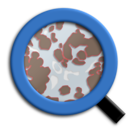
\includegraphics[height=0.35cm,valign=c]{QuPath.png}}
\newcommand{\biapyicon}{
\includegraphics[height=0.35cm,valign=c]{biapy.png}}
\newcommand{\trackmateicon}{
\includegraphics[height=0.35cm,valign=c]{trackmate.png}}


% Symbols
\newcommand{\tick}{\emoji{check-mark-button}}
\newcommand{\cross}{\emoji{cross-mark}}
\newcommand{\maybe}{\emoji{yellow-circle}}
\newcommand{\unknown}{\emoji{red-question-mark}}
\newcommand{\na}{\dots}
\newcommand{\twod}{\(_\text{2D}\)}

\begin{document}

\renewcommand{\arraystretch}{1.4}
\begin{minipage}{20cm}
\begin{tabular}{l||c c c | c || c c c}
\hline\hline
\textbf{Image Analysis} & \multicolumn{3}{c|}{\textbf{DL: The usual suspects}} & \textbf{ML} & \multirow{2}{*}{\textbf{3D}} & \multirow{2}{*}{\textbf{Time}} & \multirow{2}{*}{\textbf{Large images}} \\
\cline{2-4}
\textbf{Platforms} ↓ & \textbf{Cellpose} & \textbf{StarDist} & \textbf{InstanSeg} & \textbf{Pixel Classification} & & & \\
\cline{2-4}
& (cells, generalist) & (Nuclei) & & (Any) & & & \\
\hline\hline
\fijiicon\ Fiji  (21+)     & \tick & \na   & \cross & \tick & \cross & \tick & \cross \\
\ilastikicon\ Ilastik & \cross & \cross & \cross & \tick & \tick & \tick & \tick\twod \\
\icyicon\ Icy 3       & \tick & \maybe & \cross & \unknown & \tick & \tick & \tick\twod \\
\qupathicon\ QuPath   & \tick\footnotesize{+ fine-tuning} & \tick & \tick & \tick & \cross & \cross & \tick\twod \\
\biapyicon\ BiaPy     & \cross & \cross & \cross & \cross & \tick & \tick & \tick \\
\trackmateicon\ Trackmate    & \tick & ... & \cross & \tick & \tick & \tick & \cross \\
\hline\hline
\end{tabular}
\end{minipage}

\end{document}